\documentclass[12pt, titlepage]{article}

\usepackage{booktabs}
\usepackage{tabularx}
\usepackage{hyperref}
\usepackage{float}
\usepackage{graphicx}
\hypersetup{
    colorlinks,
    citecolor=black,
    filecolor=black,
    linkcolor=red,
    urlcolor=blue
}
\usepackage[round]{natbib}

\title{SE 3XA3: Test Report\\Question Chat}

\author{Team \#14, QChat
		\\ Adit Patel - patela14
		\\ Harsh Patel - patelh11
		\\ Vrushesh Patel - patelv12
}

\date{December 06, 2017}

% \input{../Comments}

\begin{document}

\maketitle

\pagenumbering{roman}
\tableofcontents
\listoftables

\begin{table}[H]   
\caption{\bf Revision History}
\begin{tabularx}{\textwidth}{p{3cm}p{2cm}X}
\toprule {\bf Date} & {\bf Version} & {\bf Notes}\\
\midrule
12/05/2017 & 0.1 & Initial Version\\
12/06/2017 & Rev 1.0 & Final Revision\\
\bottomrule
\end{tabularx}
\end{table}

\newpage

\pagenumbering{arabic}

This document provides the results of the tests conducted for QChat. It contains the test cases and the results for the functional and non-functional requirements.  

\section{Functional Requirements Evaluation}
The following tests were performed to ensure that the software runs correctly and the user is able to use the software as per the requirements. This portion will define each test and what the domain of the results. \\

\noindent\textbf{Test-F1: Application runs on all devices} \\
\textbf{Results:} The user is able to access QChat (\href{www.qchat.online}{www.qchat.online}) on all browsers and all devices that can connect to the internet. \\
\textbf{Input:} Enter URL into web browser. \\
\textbf{Output:} Website loads and home page shown. \\

\noindent\textbf{Test-F2: Connect to class chatroom} \\
\textbf{Results:} The user is able to enter the class chatroom using the given code.  \\
\textbf{Input:} User enters given string into textbox, presses submit key to continue. \\
\textbf{Output:} Display changes and now shows the class chatroom. \\

\noindent\textbf{Test-F3: Ask Question/Answer Question} \\
\textbf{Results:} The user is able to submit a question or answer and have it show up in the class chatroom. \\
\textbf{Input:} User enters given string into the ask question or answer textbox, presses submit key to continue. \\
\textbf{Output:} Display changes and now the class chatroom shows the question the user asked or  updates the number of solutions for the question answered. \\

\noindent\textbf{Test-F4: Post anonymously} \\
\textbf{Results:} There in no trace between a submission on QChat and the user who posted it. \\
\textbf{Input:} None \\
\textbf{Output:} System does not require any form of authentication or identification to allow a user to post, anybody can visit the site from anywhere and post a comment. \\

\noindent\textbf{Test-F4: Upvote and Downvote Questions} \\
\textbf{Results:} The user is able to upvote and down questions and the new vote count reflects this.  \\
\textbf{Input:} User clicks on the upvote button to upvote, user clicks on the downvote button to downvote. \\
\textbf{Output:} The vote count updates and increases by 1 if upvoted or decreases by 1 if downvoted. \\



\section{Nonfunctional Requirements Evaluation}


\subsection{Usability and Look and Feel}
The user survey conducted: 

\begin{figure}[H]
\centering
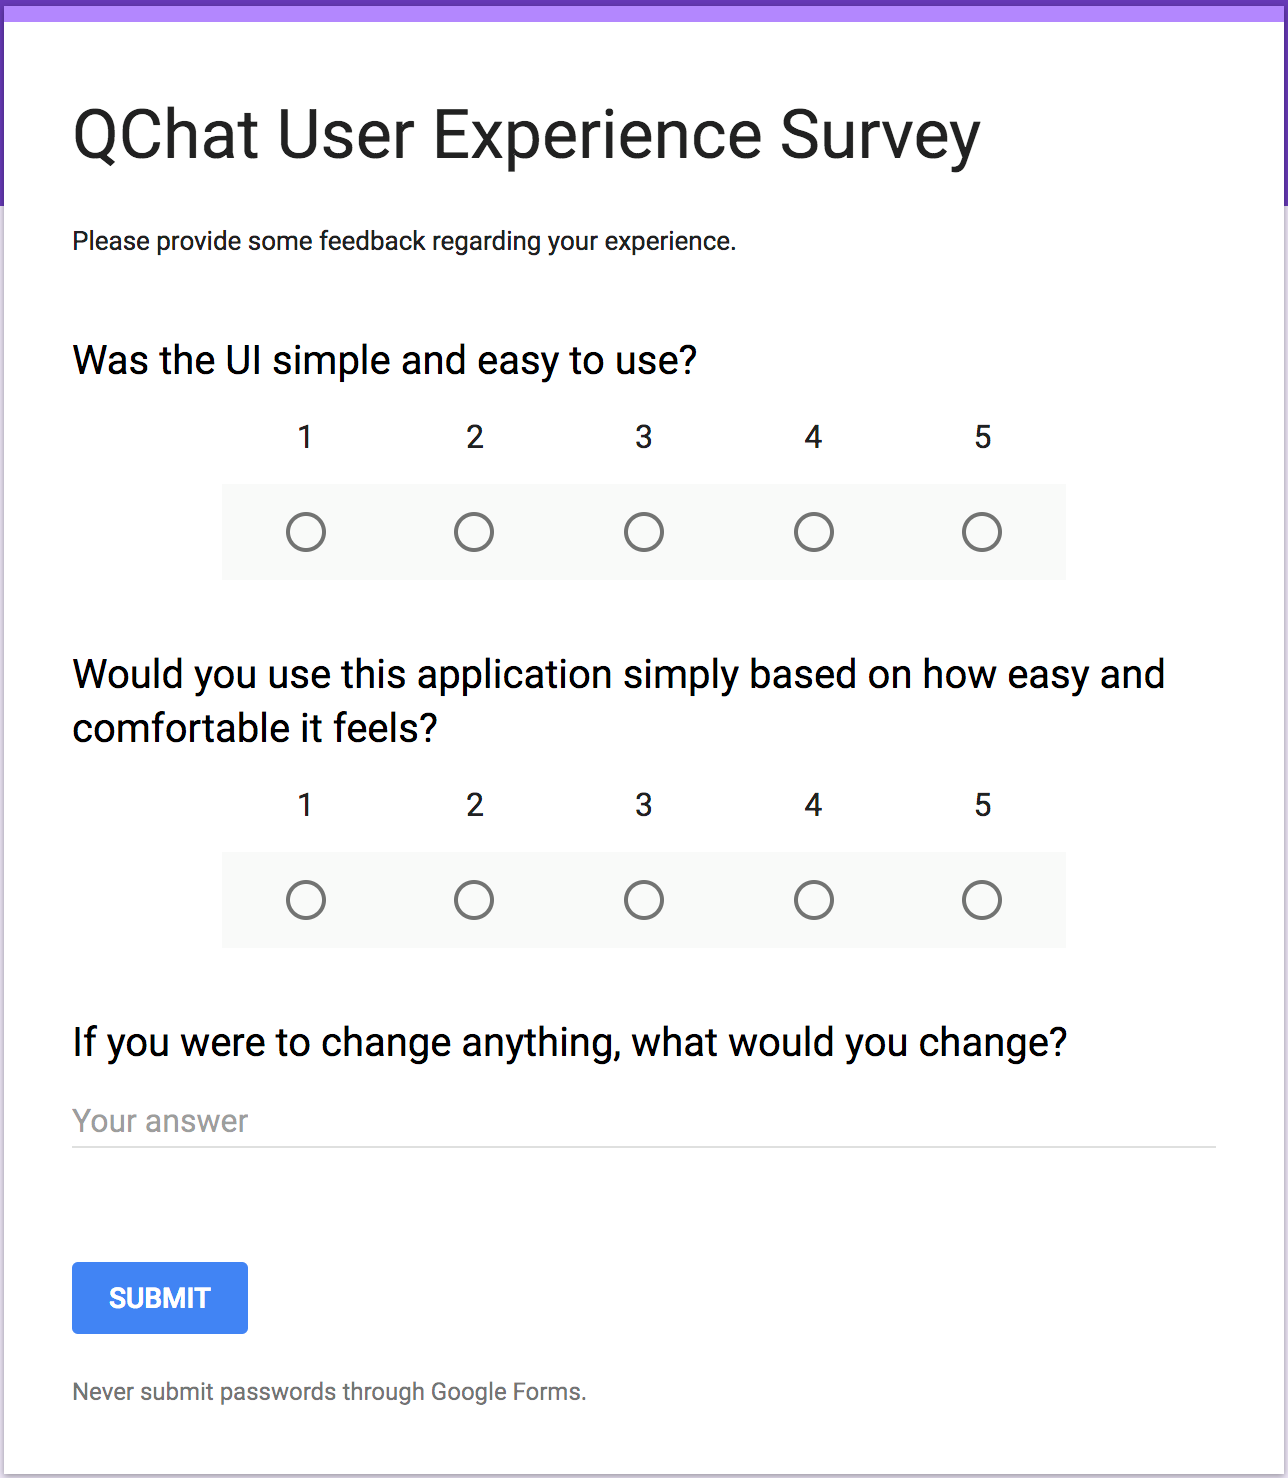
\includegraphics[width=0.63\textwidth]{Survey.png}
\caption{Use hierarchy among modules}
\label{FigUH}
\end{figure}


\textbf{Description  of Tests:} Usability and Look and Feel was tested by our colleagues at McMaster University that were from different backgrounds like Engineering, Health Science, etc. to get a better opinion on the technological experience for QChat. 	\\

\noindent\textbf{Test Name:} TestNF-1\\
\textbf{Results:} All the participants rated the look and the feel of QChat. The average was 3.9. The average was below the expected average and some feedback was received that QChat can be made to make it look like a messaging app (Ex. iMessage). \\

\noindent\textbf{Test Name:} TestNF-2\\
\textbf{Results:} The average for the responsiveness of QChat was 3.9  The average was below 4. Feedback was received that QChat can have different UI for cell phones devices. \\

\noindent\textbf{Test Name:} TestNF-3\\
\textbf{Results:} All the participants were able to use QChat without any prior instruction given. The average for the look and feel test was 4.2. The average rating was above 4 as expected which means that QChat is easy to use.  \\

		
\subsection{Performance}
\textbf{Description of Tests:} The performance of the QChat was measured by timing the actions. For example, accessing the QChat or posting a question or an answer.\\

\noindent\textbf{Test Name:} TestNF-4 \\
\textbf{Results:} The average time that the QChat take to load was 2.3 seconds. Sometimes it did take longer than 3 seconds, but mainly it was because of slow internet connection. \\

\noindent\textbf{Test Name:} TestNF-5 \\
\textbf{Results:} The average elapsed time between right after user hits send and text (question or answer) being updated on all the end users connected to same session was 1.6 seconds. The update on end user’s screen was fast, but it did take longer for sometimes when the internet connection was slow.  \\


\subsection{Operational and Portability}
\textbf{Test Name:} TestNF-6 \\
\textbf{Results:} QChat was accessible and functional on cell phones, tablets, laptops and desktops with all different OS like android, IOS, Windows, Linux and MacOS.  \\

\subsection{Maintainability}
\textbf{Test Name:} TestNF-7 \\
\textbf{Results:} The developers were able to communicate, understand and add to the code. \\

\subsection{Security}
\textbf{Test Name:} TestNF-8 \\
\textbf{Results:} QChat stores no personal data of users. Therefore, no user data was or can be compromised.  \\

\subsection{Cultural}
\textbf{Test Name:} TestNF-9 \\
\textbf{Results:} The participants did not find any vulgar text. The average was 1. \\

\subsection{Robustness}
We didn’t explicitly test robustness. Robustness was not a quality that we put within the scope of this project, however it is an important quality and it was kept in mind as we implemented and tested. The main reason robustness was not explicitly tested is because we have put adding profanity filters as future goals and the robustness of how we handle inputs can only truly be tested once these filters are in place. Otherwise our project handles any input and would indicate it is robust without even having restrictions. \\
	
\section{Comparison to Existing Implementation}	

This project did not have an open source existing implementation. We were however able to compare to  \href{https://www.sli.do/}{sli.do}. This product is a private audience interaction application which in a sense is a much more scaled product than our project. Our project does provide the same functionality at a lower scope; our project is to be used for lectures and providing a means for communication amongst students as well as with the professor. 

\section{Unit Testing}

Completed unit testing using jasmine.js.
Our group ran multiple tests that would test most of the methods defined in our JavaScript file. \\
\\
Our unit testing covered a subset of what our manual testing covered to ensure we could verify the expected results. This lead to us unit testing each of our methods.
There were some situations where we saw that unit testing certain portions of our code in smaller sections would be better. For example, testing that the integration of Firebase works was broken down and required us to manually check on Firebase console as well. \\
\\
Our unit testing verified the results that are mentioned in Functional Requirement Evaluation Section. To be specific, the tests were conducted for Test-F1 to Test-F4 only. Test-F5 was merely a visual change and could not be unit tested. 


\section{Changes Due to Testing}

After conducting usability testing surveys we realized that QChat’s initial user interface was not an intuitive to follow as we thought. Using the feedback we collected we proceeded to update the interface in a manner that everyone would understand, using the scroll view. The scroll view allowed for all our question to be organized top to bottom in a certain ordering. We also went on to hide the answers to each question instead of showing them right away as this saved space and made the class chatroom look clearer and more organized. To view anwer we added a button called “show answer” to each question and once a user was done looking at the answer the answer could be hidden again.

\section{Automated Testing}

As mentioned in our test plan, the unit testing is one of the only ways we could automate our testing. We were able to carry out these tests and successfully pass them.\\
\\
In our test plan, we mentioned that we could look into writing a script that accesses the Firebase database and reads/writes to verify that it up and working automatically. We realized that did not fit the scope of our project and decided we would allocate our resources better. 

\section{Trace to Requirements}

\subsection{Test trace to Functional Requirements}

\textbf{NOTE:} Refer to SRS to see the Requirements\\

\begin{table}[!h]
\centering
\begin{tabular}{p{0.4\textwidth} p{0.6\textwidth}}
\toprule
\textbf{Test} & \textbf{Requirements}\\
\midrule
Test-F1:  & Req-F2 \\
Test-F2:  & Req-F3   \\
Test-F3:  & Req-F1 \\
Test-F4:  & Req-F1 \\
Test-F5:  & Req-F4 \\
\bottomrule
\end{tabular}
\caption{Trace Between Requirements and Tests}
\label{TblRT}
\end{table}


\subsection{Test trace to Non-Functional Requirements}

\textbf{NOTE:} Refer to SRS to see the Requirements\\

\begin{table}[!h]
\centering
\begin{tabular}{p{0.4\textwidth} p{0.6\textwidth}}
\toprule
\textbf{Test} & \textbf{Requirements}\\
\midrule
TestNF-1:  & Usability and Look and Feel \\
TestNF-2:  & Usability and Look and Feel   \\
TestNF-3:  & Usability and Look and Feel\\
TestNF-4:  & Performance \\
TestNF-5:  & Performance \\
TestNF-6:  & Operational and Portability \\
TestNF-7:  & Maintainability \\
TestNF-8:  & Security \\
TestNF-9:  & Cultural \\
\bottomrule
\end{tabular}
\caption{Trace Between Requirements and Tests}
\end{table}

\section{Trace to Modules}	

\begin{table}[H]
\centering
\begin{tabular}{p{0.4\textwidth} p{0.6\textwidth}}
\toprule
\textbf{Test} & \textbf{Modules}\\
\midrule
Test-F1:  & M1, M2, M3, M4, M5, M6 \\
Test-F2:  & M3, M4, M5, M6   \\
Test-F3:  & M2, M4, M5, M6 \\
Test-F4:  & M2, M4, M5, M6 \\
Test-F5:  & M2, M4, M5, M6 \\
TestNF-1:  & M4 \\
TestNF-2:  & M2, M3, M5  \\
TestNF-3:  & M4 \\
TestNF-4:  & M5 \\
TestNF-5:  & M6 \\
TestNF-6:  & M1, M2, M3, M4, M5, M6 \\
TestNF-7:  & M2, M3, M4, M5, M6 \\
TestNF-8:  & M3, M5 \\
TestNF-9:  & M6 \\
\bottomrule
\end{tabular}
\caption{Trace Between Tests and Modules}
\end{table}


\section{Code Coverage Metrics}

For Qchat, the code covered in the testing is approximately 85\%. This number is based off the unit testing covering the functionality as well as manual testing which confirms the unit testing coverage as well as accesses additional code on top of it. This is evident in our trace to modules section. Along with this, we used JSLint to ensure that our all of our code followed syntax and coding guidelines for JavaScript.


\bibliographystyle{plainnat}

\bibliography{SRS}

\end{document}
